\section{Clase 1}
%\subsection{Lagrangeanos singulares y Hamiltonianos con vínculos}
Las teorías más exitosas que conocemos poseen simetrías de gauge (electrodínamica y teorías de Yang-Mills). Dichas teorías se caracterizan porque poseen \textit{vínculos}.

Las simétrias de gauge son simetrias que actuan sobre los campos localmente.

Las teorías que possen \textit{simetrías de gauge} son sistemas físicos con \textit{vínculos.}

Una caracteristica que poseen en común estas teorías es que están descritas mediante más variables que grados de libertad físicamente independientes. Por ejemplo, la electrodinámica posee simetría de gauge, por lo tanto un sistema físico puede ser descrito por infinitos campos $A_\m $, pero en realidad la teoría tiene $2$ grados de libertad físicos. Sistemas que tiene esta propiedad son conocidos como \textit{singulares}.


Las ecuaciones de Euler-Lagange incluyen ecuaciones que representan vínculos entre las coordenadas y las velocidades, $\Phi(q_i,\dot{q}_i)=0$. Por lo tanto, no todos los grados de libertad estarán completamente determinados por las ecuaciones. 
%\textit{que la misma dinámica impone en el sistema}
A nivel Hamiltoniano, estas teorías tienen vínculos de \textit{primera clase} los cuales corresponde a los \textit{generadores} de las simetrías de gauge. Es decir, toda teoría de gauge implica una teoría con vínculos, pero el recíproco no es verdad,

\begin{equation}
  \boxed{\text{Teorías de gauge} \implies \text{Teorías con vínculos}}.
\end{equation}


\subsection{Invariancia de gauge y vinculos}
Una teoría de gauge podría ser pensada como una teoría en que las variables dinámicas son especificadas con respecto a un sistema de referencia cuya eleccción es arbitraria para cada instante de tiempo. Las variables físicamente importantes son aquellas que son independientes del sistema de referencia local. Una transformación de las variables inducidas por un cambio arbitrario en el marco de referencia es conocida como una \textit{transformación de gauge}.


\begin{wrapfigure}{r}{0.4\textwidth}
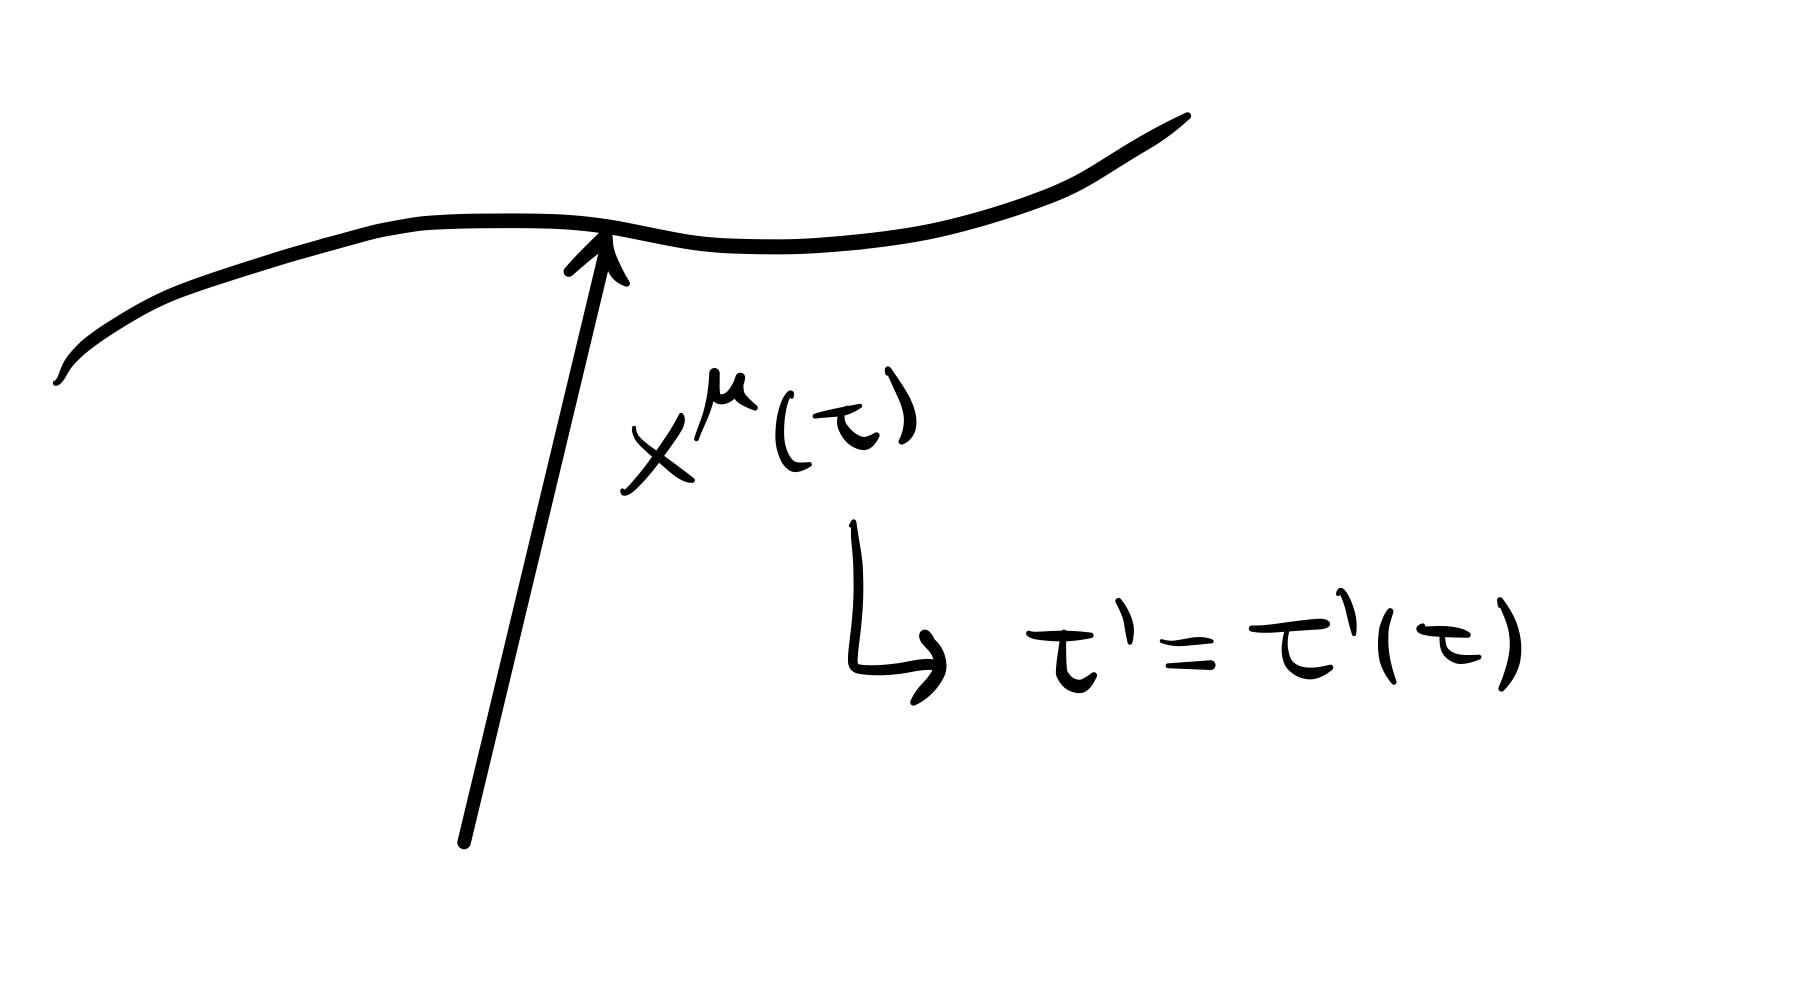
\includegraphics[width=1.0\linewidth]{1-particula} 
\end{wrapfigure}
Las varibles físicas (observables) son aquellas que son invariantes bajo transformaciones de gauge.



\begin{ej}


	Consideremos la trayectoria de una partícula relativista.
	
	En este caso la trayectoria de la partícula $x^\m$ es el campo dinámico, $\t $ es el parámetro propio relacionado con el sistema de referencia y $\t' $ es una reparametrización del parámetro propio.
	
	Consideremos una tranformación infinitesimal
	\begin{equation}
  \t'=\t +\epsilon(\t ),
\end{equation}
la cual induce una transformación de gauge sobre los campos  de la forma
\begin{equation}
  \d x^\m =-\epsilon (\t )\dot{x}^\m,
\end{equation}
y el observable corresponde a la longitud de arco $S$.
\end{ej}


En una teoría de gauge, uno no puede esperar que las ecuaciones de movimiento determinen todas las variables para todo tiempo. A partir de las misma ecuaciones iniciales, se producirán evoluciones temporales diferentes. Por lo tanto, una propiedad clave de una teoría de gauge es que la solución general de las ecuaciones de movimiento contienen funciones arbitrarias del tiempo.

La aparición de funciones arbitrarias en la solución general de las ecuaciones de movimeinto implica, a nivel Hamiltoniano, que las variables canónicas no son todas independientes. La relación que existe entre ellas son llamadas \textit{vínculos},
\begin{equation}
  \Phi(p,q)=0.
\end{equation}

\begin{tcolorbox}
En resumen, en una teoría de gauge
\begin{itemize}
	\item existe una relación entre las ecuaciones,
	\item no todas las variables están fijas por las ecuaciones de movimiento,
	\item existen vínculos de primera clases en el Hamiltoniano.
\end{itemize}
\end{tcolorbox}

\begin{ej}
	Consideremos la siguiente acción:
	\begin{equation}
  I[\psi,A_0]=\frac{1}{2}\int\dd t\left(\dot{\psi}-A_0\right)^2
\end{equation}
\begin{enumerate}
	\item \underline{\textit{Simetría de gauge}}: Esta acción es invariante bajo las siguientes transformaciones,
	\begin{equation}
  \psi'=\psi+\epsilon(t),\qquad A_0=A_0+\dot{\epsilon}(t)
\end{equation}
es directo ver que
\begin{equation}
  \d\psi=\epsilon(t),\quad \d A_0=\dot{\epsilon}(t)
\end{equation}
En efecto, la variación de la acción queda,
\begin{align}
  \d I&=\frac{1}{2}\int\dd t\left(\dv{t}(\d\psi)-\dot{\epsilon}(t)\right)^2\\
  &=\frac{1}{2}\int\dd t\left(\dot{\epsilon}(t)-\dot{\epsilon}(t)\right)^2\\
  &=0
\end{align}
donde $\epsilon(t)$ es arbitrario.

\item \underline{\textit{Las ecuaciones de movimiento no son independientes}}:
\begin{equation}
  \frac{\d I}{\d A_0}=0\implies (\dot{\psi}-A_0)=0
\end{equation}
\begin{equation}
  \frac{\d I}{\d \psi}=0\implies 2\left(\dot{\psi}-A_0\right)\dv{t}(\d\psi)=0\implies \dv{t}(\dot{\psi}-A_0)=0
\end{equation}
Es fácil ver que ambas ecuaciones son diferencialmente dependientes.
\item \underline{\textit{La solución más general contiene funciones arbitrarias}}: La solución más general para este sistema de ecuaciones será,
\begin{align}
  \psi(t)&=f(t)\\
  A_0(t)&=\dot{f}(t)
\end{align}
Por lo tanto, implica una función arbitraria.

Independiente de cuales seal las condiciones iniciales, uno siempre puede modificar la evolución en un tiempo posterior.

\item \underline{\textit{El Hamiltoniano posee vínculos}}. Para pasar a la formulación Hamiltoniana, calculamos las momentas,
\begin{align}
  P_{A_0}&=\pdv{L}{\dot{A_0}}=0\\
  P_{\psi}&=\pdv{L}{\dot{\psi}}=\left(\dot{\psi}-A_0\right)
\end{align}
Luego, el Hamiltoniano queda
\begin{align}
  H&=P_\psi \dot{\psi }-L\\
  &=P_\psi(P_\psi+A_0)-\frac{P_\psi^2}{2}\\
  &=\frac{P_\psi^2}{2}+P_\psi A_0
\end{align}
Escribimos la acción Hamiltoniana
\begin{align}
  I[P_\psi,\psi,A_0]&=\int\left(P_\psi \dot{\psi}-\frac{1}{2}P^2_\psi-A_0P_\psi\right)\dd t
\end{align}
Las ecuaciones se obtienen al variar la acción respecto a $P_\psi, \psi$ y $A_0$ son equivalentes a las que se obtienen a partir del Lagrangeano. En efecto,
\begin{equation}\label{1.vinculo}
  \frac{\d I}{\d A_0}=-P_\psi=0 \qquad (\text{vínculo})
\end{equation}
Utilizamos las ecuaciones canónicas,
\begin{equation}
  \dot{\psi}=\pdv{H}{P_\psi}=P_\psi+A_0
\end{equation}
\begin{equation}\label{1.ec1}
  \implies \boxed{\dot{\psi}-P_\psi-A_0=0}
\end{equation}
\begin{equation}\label{1.ec2}
  \boxed{\dot{P}_\psi=-\pdv{H}{\psi}=0}
\end{equation}

Notemos que \eqref{1.vinculo} es considerado un vínculo debido a que corresponde a una restricción sobre coordenadas del espacio de fase. Es decir, estamos restringinedo las ecuaciones dinámicas \eqref{1.ec1} y \eqref{1.ec2} sobre una superficie en el espacio de fase dada por dada por $P_\psi=0$.

\end{enumerate}
\end{ej}





































